\documentclass[handout, 10pt]{beamer}

%\usepackage[backend=bibtex,firstinits=true,style=verbose-inote,citestyle=authortitle]{biblatex}
\usepackage{bm}
\usepackage{graphicx}
\usepackage{subcaption}
\usepackage{amsmath}
\usepackage{amsfonts}
\usepackage{makecell}
\usepackage{filecontents}
\usepackage{biblatex}
% \newcommand{\expect}[2][]{
\ifthenelse{\equal{#1}{}}{
\mathbb{E}\left[#2\right]
}{
\underset{#1}{\mathbb{E}}\left[#2\right]
}}

\newcommand{\cov}[2][]{
\ifthenelse{\equal{#1}{}}{
\text{Cov}\left[#2\right]
}{
\underset{#1}{\text{Cov}}\left[#2\right]
}}


\newcommand{\var}[2][]{
\ifthenelse{\equal{#1}{}}{
\text{Var}[#2]
}{
\underset{#1}{\text{Var}}[#2]
}}

\newcommand{\loss}[2][]{
\ifthenelse{\equal{#1}{}}{
\mathcal{L}(#2)
}{
\mathcal{L}_{#1}(#2)
}}

\newcommand{\kl}[2]{
\text{D}_\text{KL}[#1 \parallel #2]
}

\newcommand{\R}{\mathbb{R}}
%\newcommand{\Prob}{\mathbb{P}}

\newcommand{\1}[1]{\mathds{1}\{#1\}}


%\usecolortheme{dolphin}
\setbeamertemplate{navigation symbols}{}
\setbeamertemplate{section in toc}{\inserttocsectionnumber.~\inserttocsection}

\begin{filecontents*}{references.bib}
@InProceedings{SinGAN,
author = {Shaham, Tamar Rott and Dekel, Tali and Michaeli, Tomer},
title = {SinGAN: Learning a Generative Model From a Single Natural Image},
booktitle = {The IEEE International Conference on Computer Vision (ICCV)},
month = {October},
year = {2019}
}
\end{filecontents*}

\addbibresource{references.bib}


\title{SinGAN: Learning a Generative Model from a Single Natural Image\footnote{\citepaper{SinGAN}}}
%\subtitle{}
%\author{Ivan Skorokhodov}
%\date{}
%\logo{
\includegraphics[height=1cm]{images/ipavlov-logo.png}}

\newcommand{\citepaper}[1]{\citetitle{#1} by \citeauthor{#1}}

%\graphicspath{{./images}}

%\usetheme{lucid}
\begin{document}

\begin{frame}
    \titlepage
\end{frame}

\begin{frame}{Overview}
    \begin{figure}
        \centering
        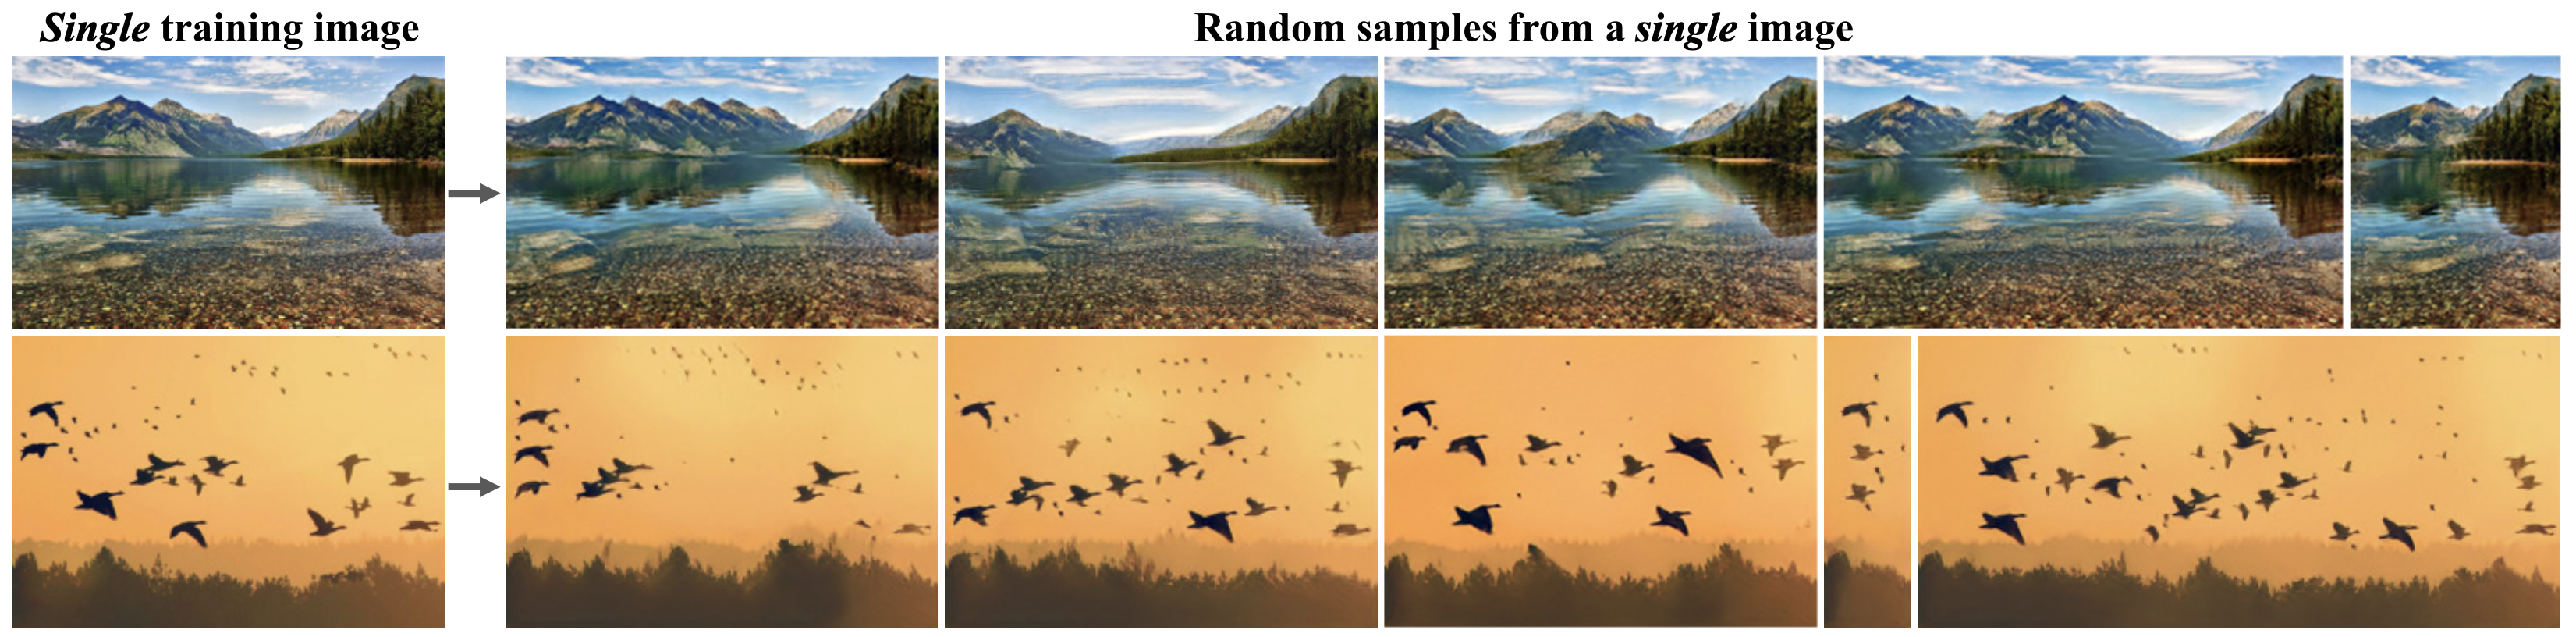
\includegraphics[width=\textwidth]{images/singan-main-samples.png}
    \end{figure}
    
    \begin{itemize}
        \item\pause \textbf{SinGAN} is a GAN model which is trained on a \textit{single} image and can generate similar ones.
        \item\pause It does so by using a Pyramid of GAN models, starting with a small resolution and gradually increasing it.
        \item\pause Authors obtained \textit{very} good results on other generative tasks: super-resolution, paint to image, editing, etc.
    \end{itemize}
\end{frame}

\begin{frame}{SinGAN in short}

\begin{itemize}
    \item\pause Take an image and downsample it several times to obtain a sequence $x_0 > x_1 > ... > x_N$ of its downsampled versions.
    \item\pause Initialize $N$ GANs $(G_0, D_0), ..., (G_N, D_N)$, where $(G_n, D_n)$ operate on image resolution of $x_n$.
    \item\pause On each level $n$, generator takes an image $\tilde x_{n-1}$ from the previous level and produces an image for the next level: $\tilde x_n = G_n(z_n, \tilde x_{n-1})$.
    \item\pause In addition to an adversarial loss, we also use a reconstruction loss to reconstruct original image.
\end{itemize}

\end{frame}

\begin{frame}{Architecture}
    \pause
    \begin{figure}
        \centering
        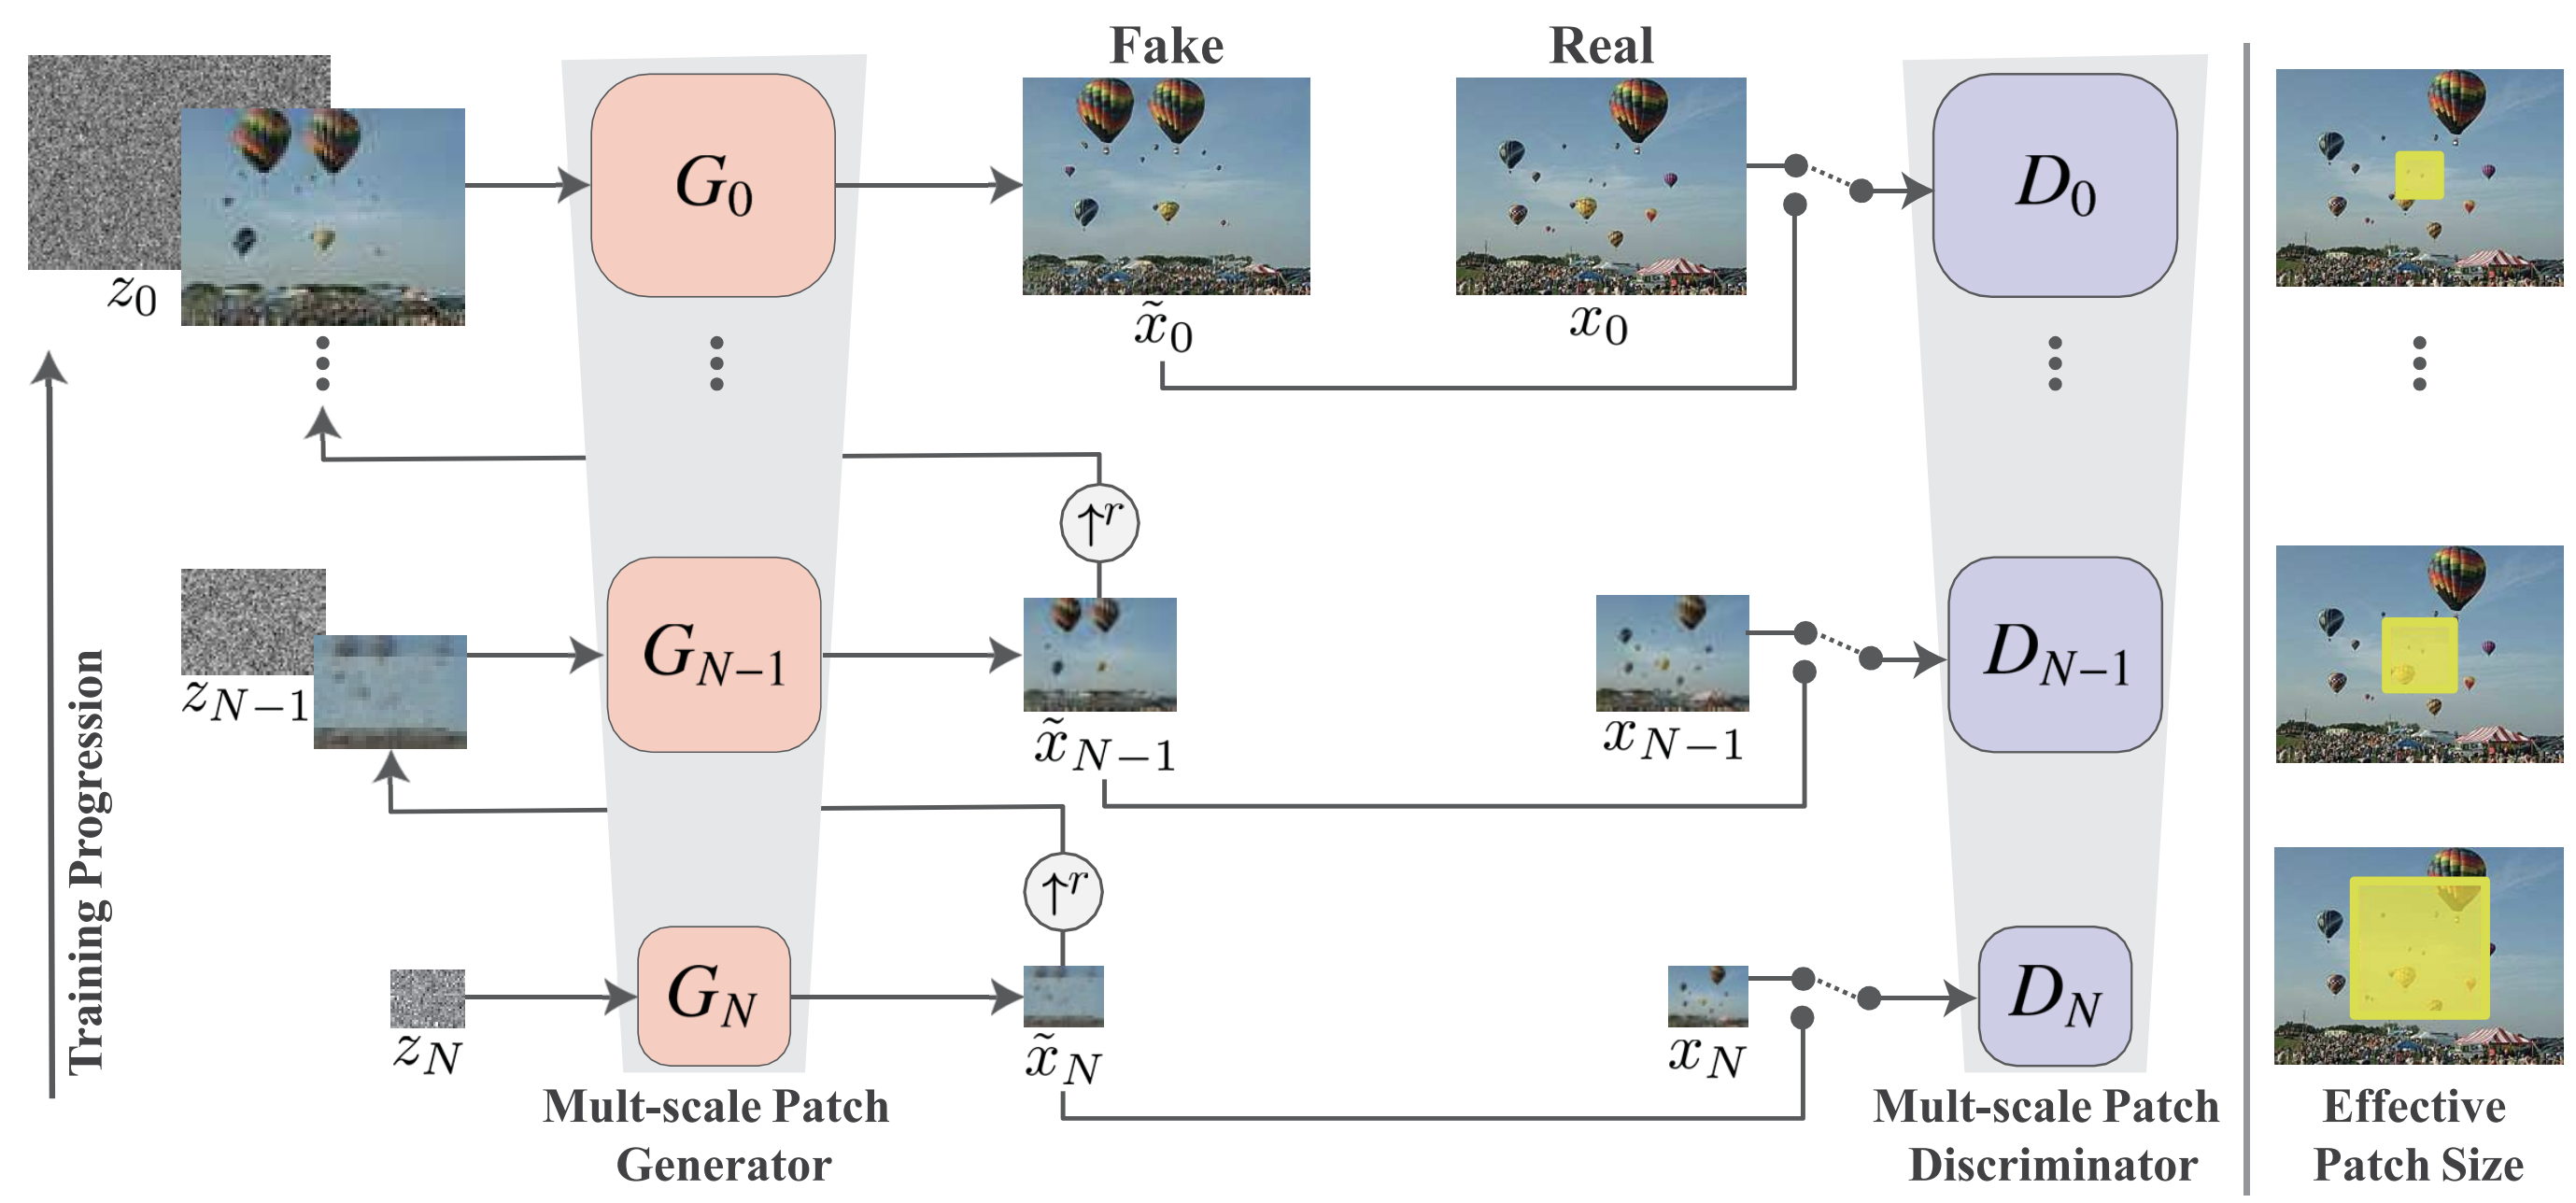
\includegraphics[width=\textwidth]{images/singan-architecture.png}
    \end{figure}
    
    \begin{itemize}
        \item\pause On each level, we take noise $z_n$ and image from the previous level $\tilde x_{n+1}$ and generate image $\tilde x_n = G_n(z_n, \tilde x_{n+1})$.
        \item\pause Discriminator $D_n$ works on patches instead of the full image scale.
    \end{itemize}
\end{frame}

\begin{frame}{Architectural details}
    \begin{itemize}
        \item\pause Given noise $z_n$ and upsampled previous image $\tilde x_{n+1}^\uparrow$, generator $G_n$ predicts only ``missing details'' which we should add to an image, i.e. we do not predict the image from scratch.
        \item\pause To incorporate noise, we just some it up: $z_n + \tilde x_{n+1}^\uparrow$ (this forces $G_n$ not to discard it)
        \begin{figure}
            \centering
            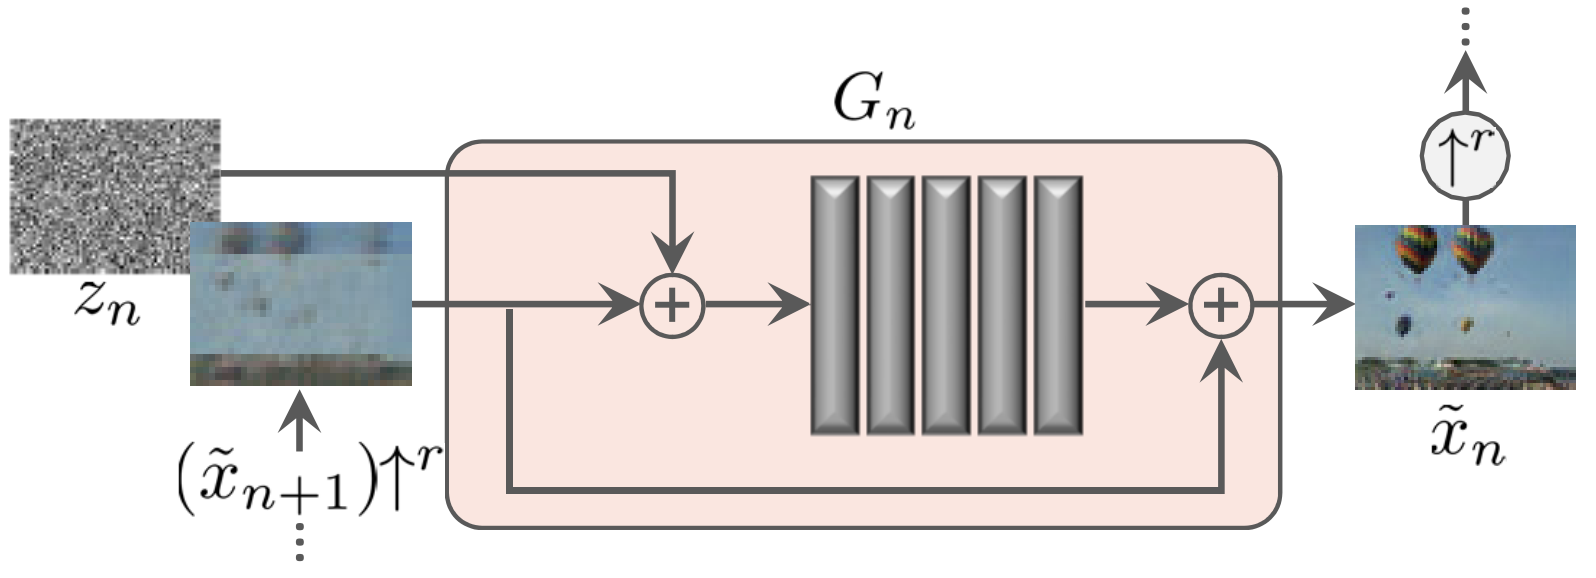
\includegraphics[width=0.5\textwidth]{images/singan-generator.png}
            \caption{Generator architecture}
        \end{figure}
        \item\pause Discriminator $D_n$ operates on patches of images instead of their full scales
        \item\pause $G_n, D_n$ are kept simple so not to overfit.
    \end{itemize}
\end{frame}

\begin{frame}{Training details}
    \begin{itemize}
        \item\pause The whole architecture is trained sequentially, i.e. once the $(G_n, D_n)$ is trained, it is kept fixed.
        \item\pause Adversarial loss:
        \begin{itemize}
            \item\pause Adversarial loss $\mathcal{L}_{\mathrm{adv}}$ is WGAN-GP loss
            \item\pause They used PatchGAN (or ``markovian discriminator''), which predicts scores for image patches independently and the final score for an image is an average of individual patch scores.
        \end{itemize}
        \item\pause Reconstruction loss:
        \begin{itemize}
            \item\pause We want to ensure that our model can produce an original image for some noise vector.
            \item\pause Pick ``golden'' noise vectors $z_N^\text{rec}, z_{N-1}^\text{rec}, ..., z_0^\text{rec}$ to be $z^*, 0, ..., 0$, where $z^*$ is random and fixed.
            \item\pause Force $G_n$ to produce original (downsampled) image $x_n$ from the given noise $z_n^\text{rec}$ and previous reconstruction $\tilde{x}_{n+1}^{\mathrm{rec}}$ by optimizing:
            \begin{equation}
\mathcal{L}_{\mathrm{rec}}= \|G_{n}(0,\left(\tilde{x}_{n+1}^{\mathrm{rec}}\right)^\uparrow)-x_{n} \|^{2}
\end{equation}
        \end{itemize}
        \item\pause Total loss: 
        \begin{equation}
\min _{G_{n}} \max _{D_{n}} \mathcal{L}_{\mathrm{adv}}\left(G_{n}, D_{n}\right)+\alpha \mathcal{L}_{\mathrm{rec}}\left(G_{n}\right)
\end{equation}
    \end{itemize}
\end{frame}

\begin{frame}{Image manipulation with SinGANs}
SinGAN gives a straightforward way to do different image manipulations after training \textit{without any additional tuning}:
    \begin{itemize}
        \item\pause Super-resolution: just apply $G_0$ several times to a low-resolution image.
        \item\pause Paint to image (create an image from a clip art): downscale clip-art image to the coarsest scale and feed it to $G_N$.
        \item\pause Harmonization (blend a pasted object with a background): downscale the image to a factor $n \approx 3$ and feed it to $G_n$.
        \item\pause Editing (replace image regions): same as for harmonization.
    \end{itemize}
\end{frame}

\begin{frame}{Image manipulation samples}
    \begin{figure}
        \centering
        \includegraphics[width=\textwidth]{images/singan-image-manipulation.png}
    \end{figure}
\end{frame}

\begin{frame}{Harmonization samples}
    \begin{figure}
        \centering
        \includegraphics[width=\textwidth]{images/singan-image-manipulation-van-gogh.png}
    \end{figure}
\end{frame}


\begin{frame}{Conclusion}
    \begin{itemize}
        \item Good quantitive results on standard metrics and human evaluation
        \item A possibility to train a good GAN model from a single image gives a lot of opportunities.
        \item Previous works on single-image GANs were only about producing texture
        \item Good results on image manipulation
        \item Ablation study is missing
        \item How will we benefit from using several images?
    \end{itemize}
\end{frame}

\end{document}
